%\documentclass[letterpaper,twocolumn,10pt]{article}
\documentclass{cls/sig-alternate-10pt}

\setlength{\pdfpagewidth}{8.5in}
\setlength{\pdfpageheight}{11in}

\usepackage{amsmath,amssymb}
\usepackage{times}
\usepackage{xcolor}
\usepackage{graphics}
\usepackage{xspace}
\usepackage{amsmath, amssymb}
\usepackage[hyphenbreaks]{breakurl}
\usepackage[hyphens]{url}
\usepackage{hyperref}
\usepackage{subfigure}
\usepackage[font=bf,labelfont=bf]{caption}

\newcommand{\tabincell}[2]{\begin{tabular}{@{}#1@{}}#2\end{tabular}}
\newcommand{\summation}[2]{\ensuremath{\displaystyle\sum\limits_{#1}^{#2}}}
\newcommand{\rbr}[1]{\left(#1\right)}
\newcommand{\cbr}[1]{\left\{#1\right\}}

\renewcommand\textfloatsep{0.05in}
\renewcommand\abovecaptionskip{0.05in}
\renewcommand\belowcaptionskip{0.05in}
\renewcommand\dbltextfloatsep{0.05in}

\def\todo#1{{\textcolor{red}{TODO: {\sf #1}}}}
\def\ratul#1{{\textcolor{blue}{ratul: {\sf #1}}}}
\def\harry#1{{\textcolor{purple}{harry: {\sf #1}}}}
\def\aditya#1{{\textcolor{cyan}{aditya: {\sf #1}}}}
\def\raajay#1{{\textcolor{green}{raajay: {\sf #1}}}}
\def\matt#1{{\textcolor{orange}{matt: {\sf #1}}}}

\def\para#1{\vspace{0.05in}\noindent\textbf{#1}\hspace{0.1in}}

\newcommand{\sysname}{{\small {\sf Footprint}}\xspace}
\newcommand{\sysnamesec}{{\sf Footprint}\xspace}
\newcommand{\myeqn}[1]{{\small $#1$ \normalsize}}

\newcommand{\anycast}{{\small {\sf WAN-TE}}\xspace}
\newcommand{\disjoint}{{\small {\sf Disjoint}}\xspace}
\newcommand{\fpbasic}{{\small {\sf JointBasic}}\xspace}
\newcommand{\fptemporal}{{\small {\sf JointTemporal}}\xspace}
\newcommand{\oracle}{{\small {\sf Oracle}}\xspace}

\begin{document}

\title{Abstract RDMA}

\date{}


\maketitle
\thispagestyle{empty}

\textbf{Abstract---} 
With the tremendous popularity gained by container technology, many applications are being containerized:
splitting into numerous containers connected by networks. However, current container networking solutions
have either bad performance or poor portability, which undermines the advantages of containerization.
In this paper, we propose \sysname, a container networking solution which achieves both high performance
and good portability. \sysname is designed according to the observation that strict isolations are unnecessary 
among containers trusting each other, and it can significantly boost the communication quality of containers by 
compromising isolation a little bit. Specifically, we enable containers on the same physical machine
to communicate via shared-memory and the ones on different physical machines communicate via
high performance networking options, e.g. RDMA and DPDK. Naively wrapping up all the solutions
together will result in poor potability of containers and huge complexity in application development.
Instead, \sysname leverages a network abstraction which supports all common network APIs and 
a centralized network orchestrator which decides how to deliver data transparently to applications in the containers.
\section{Introduction} 
\label{sec:introduction}

\begin{quote}
{\em 
The history of all hitherto computer science is (often) the history of a
struggle between isolation, portability and performance. \\ 
(With apologies to Karl Marx.)}
\end{quote}

At the dawn of computing, applications had access to (and had to manage) raw
hardware. Applications were not portable, and isolation between
applications was non-existent. As operating systems emerged, they offered a modicum 
of isolation and portability.  As users demanded more portability and better
isolation between applications, operating systems became more sophisticated,
and deep layering became the norm; e.g., the modern TCP/IP stack is a classic
example of this trend.  Layering improves the application's portability across
systems and types of  networks, but incurs well-known performance
issues~\cite{dcqcn,luigipapers}. The trend continued with virtualization, which offers even more isolation, and
additional portability (e.g., you can pack up and move VMs at will, even live-migrate
them). In return, performance -- especially the network performance is further
reduced~\cite{}, and requires any number of hacks to pierce through the
isolation boundary enforced by the hypervisor to offer better performance (e.g.,~\cite{sriov,netvm,netmap,dpdk}).


%, and offers a certain
%degree of isolation applications 

%The deep layering
%significantly improves the application's portability (the same code can be reused
%on many systems and on many types of physical networks), and offers a certain
%degree of isolation applications (via mechanisms like rate control or firewalls
%implemented in the kernel). 
%However, this very same layering makes the modern TCP/IP stack greatly
%inefficient~\cite{dcqcn,luigipapers}.  \vyas{i would suggest shrinking this para even more  .. this might lead people 
%to think we are doing dpdk/megapipe style things} 
%In each case, as the impact of the performance drop was felt, new techniques
%were devised to improved performance by sacrificing some portability and
%isolation.  For example, kernel-bypass techniques such as Remote Direct Memory Access (RDMA) and
%DPDK \cite{dpdk} completely bypass the TCP/IP stack improve performance, but reduce
%portability (the code can only run on certain hardware) and offer less isolation
%(the application is more exposed to hardware vagaries, and kernel cannot provide
%protections like rate limiting and firewalls). In case of virtualization,
%techniques like SR-IOV \cite{sriov} and NetVM~\cite{netvm} pierce through the
%isolation boundary enforced by the hypervisor to offer better performance. 


The latest step in this trend is {\em containerization}~\cite{XXX}.  By wrapping a process
into a complete filesystem and namespace cell, a container has everything needed
to run the process, including executables, libraries and system tools.  A
container has no external dependencies, which makes it highly portable. The
namespace of the container is isolated from other containers, eliminating
worries about naming and version conflicts.  Such portability and independence
significantly simplifies the life cycle of a containerized application, from
testing to high availability maintenance. 
%\vyas{ideally i want containerization to appear in para 2 .. the rest is a bit too 
% much scaffolding IMO} 

%However, this isolation and portability comes at the cost of performance. 

\begin{figure}[th]
     \centering 
     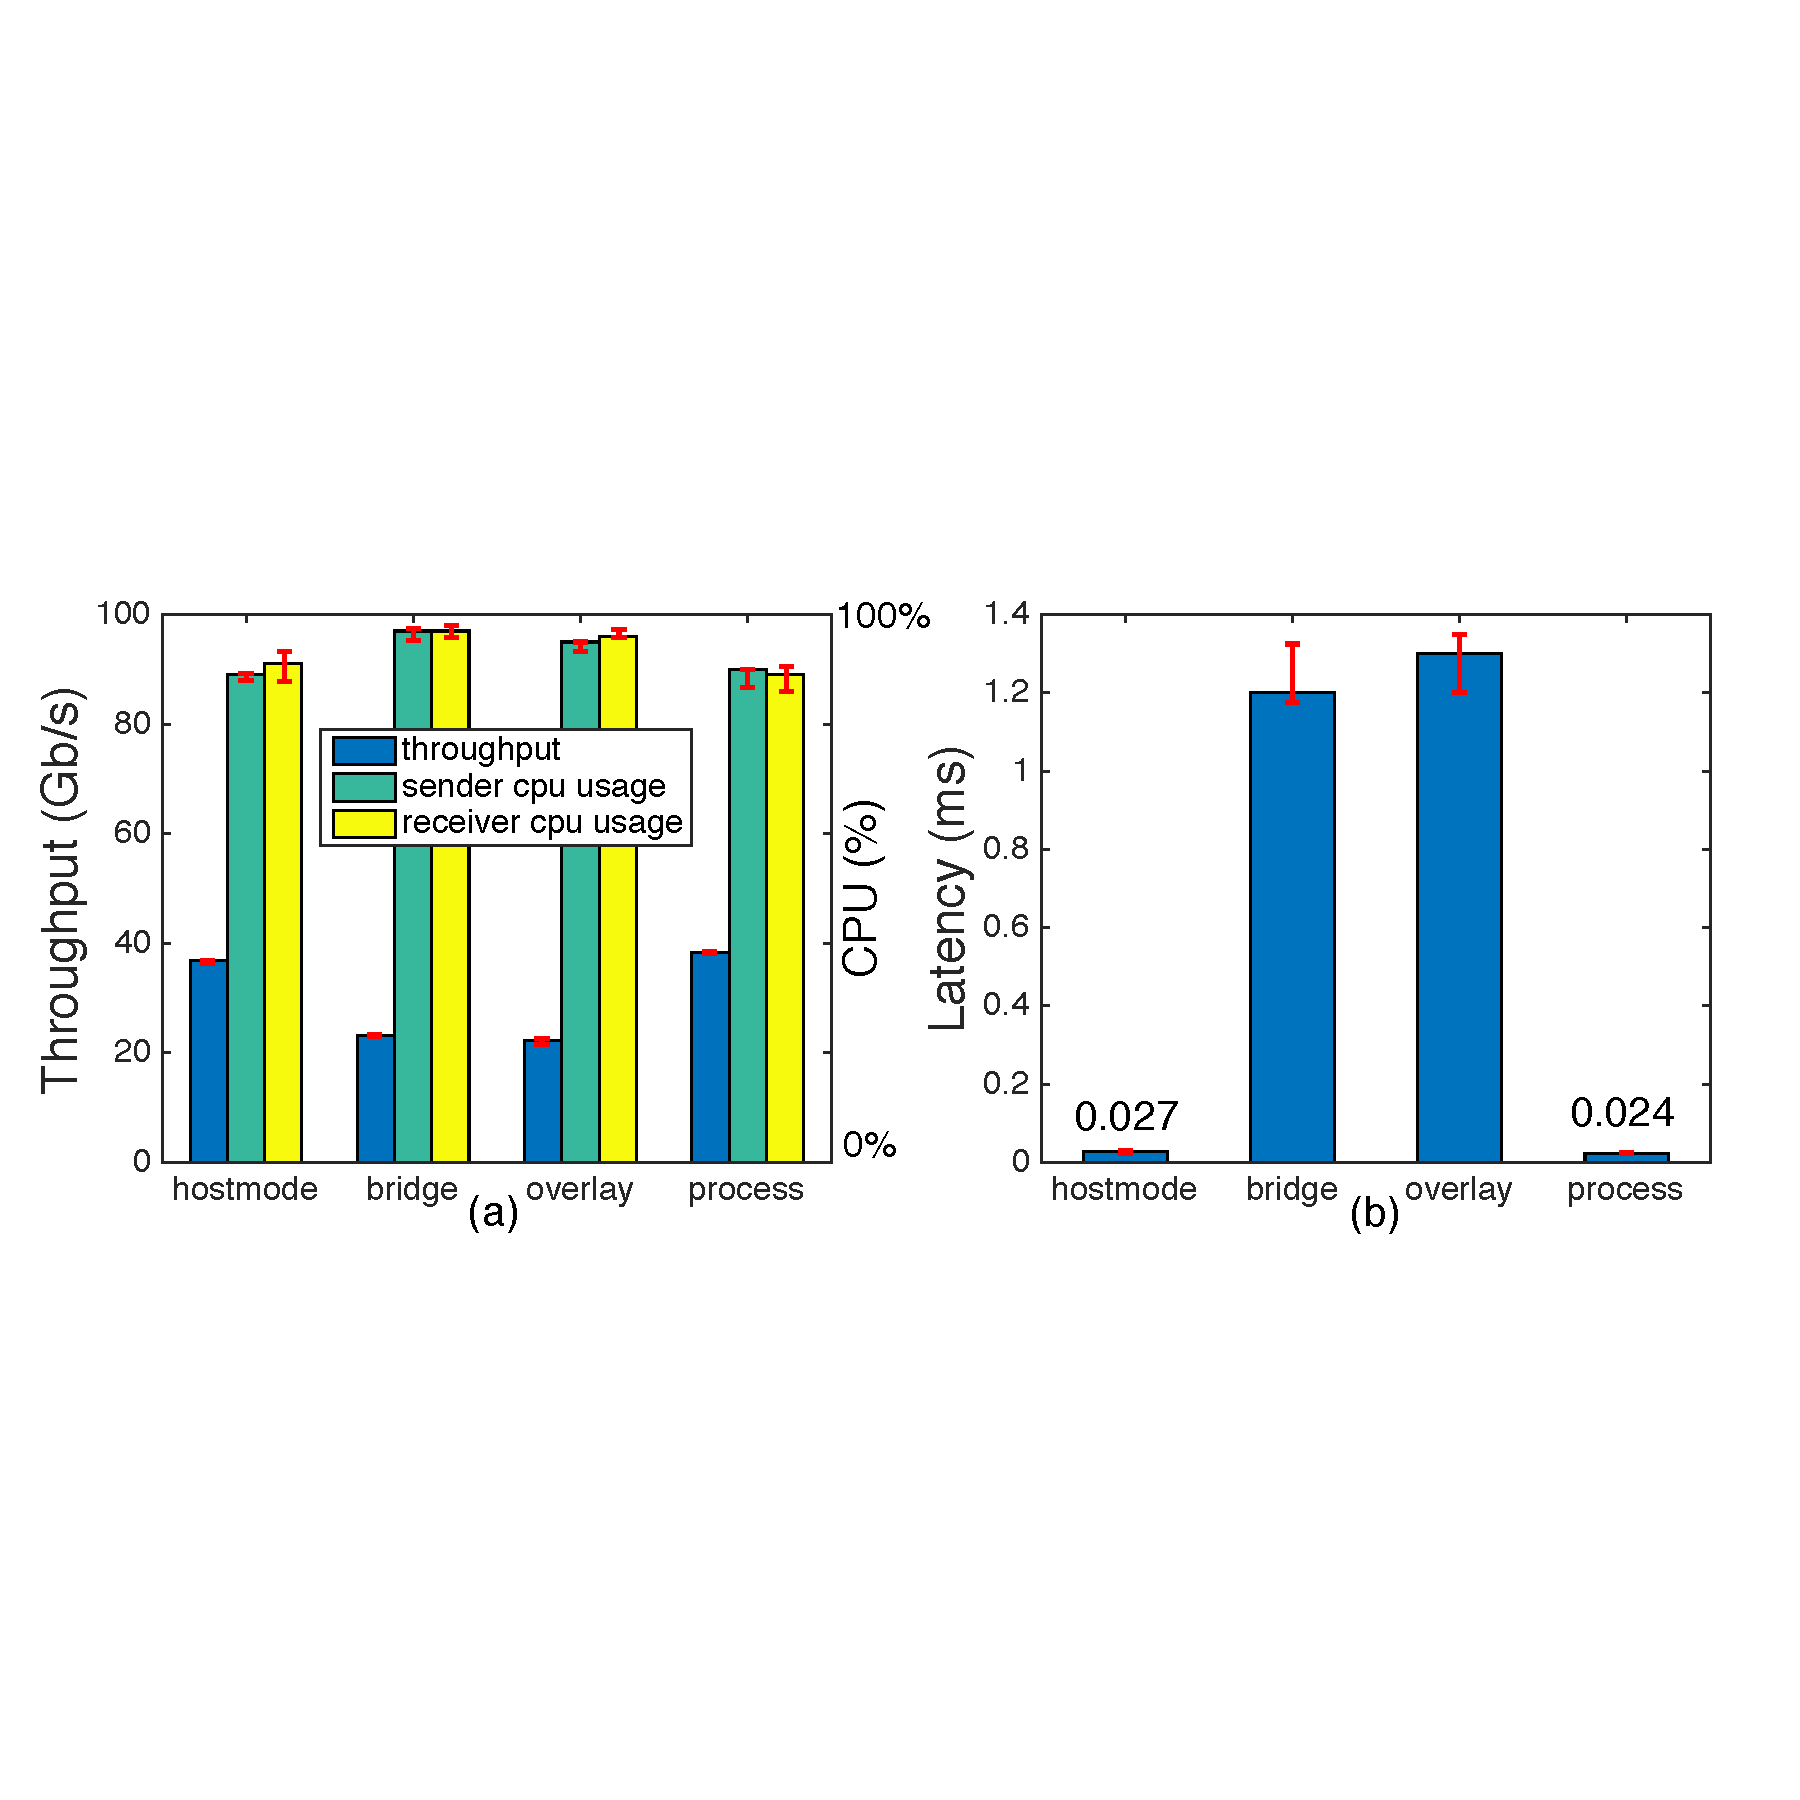
\includegraphics[width=0.5\textwidth]{figures/intro/intro_exist2.pdf} 
     \caption{Performance of two modes of container networking, compared to
     shared memory IPC.} 
     \label{fig:three_modes} 
\end{figure} 
 Unfortunately, containers too suffer the veritable curse of having 
 to sacrifice performance at the expense of isolation and portability. 
 To understand these potential performance bottlenecks, we set up a simple experiment (more details in Section~\ref{sec:motivation}).  
 We set up two Docker containers on a
server (Intel Xeon 2.40GHz 4-cores CPU, 67 GB of memory, 40Gbps Mellanox CX3
NIC, CentOS 7). We consider three ways for the containers to communicate with
each other: (1) {\em Shared Memory:} This requires special setup,
to bypass the namespace isolation, and offers the least isolation, and the least portability;
 (2) {\em Host  mode} 
in which one container binds an interface and a port on the host and use the
host's IP to communicate, like an ordinary process and hence 
 are not truly isolated as they must share the port space; and (3)  {\em Overlay mode} in which the host runs a software
router which connects all containers on the host via  a bridge network and the software routers enable 
 overlay routing across multiple hosts to enable maximum portability as  each container can even have public IPs assigned.
% to
%achieve a uniform IP assignment and traffic routing on the overlay. This makes
%containers fully portable -- they can even have public IPs assigned to them.



%We also had to write a speical application
%that used the shared memory IPC calls for communication. This mode of
%communication offers the least isolation, and the least portability. 

%Next, we considered two networking modes. First, the so-called 
%And then, the so-called 

Figure~\ref{fig:three_modes} is a telling demonstration of the fundamental
tussle between portability, isolation, and performance. We make two
observations from this figure. First, that the throughput and latency of both
modes of inter-container communication is significantly worse than
shared-memory IPC. The reason is obvious: the container communication takes a
``hairpin'' path through the full TCP/IP stack. Second, the performance of
overlay networking is worse than host mode. The reason, again, is simple: in
case of overlay networking, hairpinning happens twice, since the packets must
traverse through the software router as well. This figure thus clearly
illustrates the performance cost of isolation and portability.

As the popularity of container networking grows, this inefficiency must be
addressed. On one hand, the low throughput and high latency directly impacts
the overall performance of large scale distributed systems, such as big data
analytics~\cite{choudhury-paper,mapreduce}, key-value store~\cite{farm,cassandra,bigtable}, machine learning,
etc.  On the other hand, it forces the applications to reserve substantial CPU
resources to merely perform traffic processing, which significantly raise the
cost of running the applications.

One may argue that there is nothing new here: virtualization suffers from
similar inefficiencies and we know how to address them using techniques like
SR-IOV~\cite{sriov} and NetVM~\cite{netvm}. Unfortunately, these ideas cannot be directly applied to the container world.
SR-IOV typically scales to tens of VMs per server. In typical deployments, there
are hundreds of containers per server. The cost of supporting so many containers
in the NIC hardware will be prohibitive.  NetVM~\cite{netvm} cannot be used
directly with containers, since it destroys portability -- it works only when
two VMs are on the same server.  Developers prize containers especially for
their portability: indeed, Docker's main selling point is that a containerized
application that runs on developer's desktop will run in the cloud without any
changes! 

%% In the above experiment, containers were on the same physical server. When
%% containers are on different physical servers, things become even trickier. For
%% example, such containers cannot easily use kernel bypass technologies like RDMA.
%% The reason is subtle: using RDMA (i.e. to bypass the kernel) direct access to
%% NICs is needed. This can only be done in the host mode -- since in the overlay
%% mode, the packets have to pass through the software router.  But operating in
%% the host mode means that containers on the same host share IP address, and must
%% carefully divvy up port space to avoid conflicts.  This limits their portability
%% -- e.g. there can be only one container bound to port 80 on each physical
%% server!

In this paper we outline a solution to address this issue.  Our ultimate vision
is to develop a container networking solution which provides high throughput,
low latency and negligible overhead and fully preserves container portability in
a manner that is completely transparent to application developers. 

To achieve these seemingly conflicting goals, we observe an opportunity to
leverage two key aspects of typical container deployments: (1) they are
typically managed by a central orchestrator (E.g., Mesos \cite{mesos} \vyas{also add kubernetes or whatever to enure this 
 is not mesos specific}) and (2) are typically
deployed over managed network fabrics (e.g., a public cloud provider). Taking
advantage of these easily available additional bits of information, we sketch a
roadmap for an overlay-based solution  with flexible IP assignment and routing
in control-plane \vyas{why is this necessary} that obtains the relevant
deployment-specific information from the aforementioned container orchestrator
and fabric manager and use this in conjunction with the "right" I/O mechanism
(e.g., shared memory when containers are co-located, vs. RDMA when they are
not). 

While this sounds conceptually simple, there are several architectural
and system design challenges in realizing this vision in practice. In the rest
of the paper, we discuss these challenges and sketch a preliminary design. We
will also present results from an early prototype.

\section{Related Work} \label{sec:related}

%NetVM  \cite{netvm}
%DPDK and NetMap \cite{netmap}

\textbf{Inter-VM Communication:} 
The tussle between isolation and performance is not unique to containers.
In the field of Inter-VM Communication, there are several works that provides
high-performance by removing some of the isolation constraints.
For example, NetVM\cite{netvm} provides a shared-memory framework that
exploits the DPDK library to provide zero-copy delivery between VMs.
Netmap\cite{netmap} and VALE\cite{vale} (which is also used by ClickOS\cite{clickos}) 
are sharing buffers and metadata between kernel and userspace to eliminate memory copies.
However, these works actually strengthened the binding between VM and underlying host
structures, thus they cannot satisfy the portability requirement for \sysname. 
Also, the NetVM work is applicable only to intra-host setting,
constrained by the possibility of shared memory. Similarly, the Netmap
and VALE solutions are sub-optimal when the VMs/containers are located
on the same physical machine.

\textbf{RDMA and HPC:} RDMA originated from the HPC world, in the form of InfiniBand. The HPC
community proposed RDMA enablement solutions for
virtualization~\cite{ranadive2012toward} and
containerization~\cite{rdmacontainers} technologies. These solutions
are addressing the challenges in exposing RDMA interfaces to
virtualized/containerized applications, treating each VM/container as
if it resides on a different node.

The HPC community have also been using shared-memory based
communication~\cite{KNEM,MPI:p:MPI,HybridMPI} for intra-node
communication. These solutions are targeting MPI processes residing on
a shared non-containerized, non-virtualized machine. They do not
attempt to pierce the virtualization/containerization for additional
performance.

The same concepts described for \sysname can also be applicable for
MPI run-time libraries. This can be achieved either by layering the
MPI implementation on top of \sysname, or by implementing a similar
solution in the MPI run-time library.

\textbf{General improvements}
%low latency socket

%http://facweb.cti.depaul.edu/jyu/Publications/Yu-Linux-TSM2004.pdf
%High performance networking using SR-IOV \cite{highsriov}


%\cleardoublepage
\bibliographystyle{abbrv}
\bibliography{all_hotnets,all}

\end{document}
